
%%%%%%%%%%%%%%%%%%%%%%%%%%%%%%%%%%%%%%%%%%%%%%%%%%%%%%%%%%%%%%%%%%%%%%%%%
%           Capítulo 3: Control               %
%%%%%%%%%%%%%%%%%%%%%%%%%%%%%%%%%%%%%%%%%%%%%%%%%%%%%%%%%%%%%%%%%%%%%%%%%

\chapter{\textcolor{Azul}{Control}}

A pesar de la existencia de robots comerciales de tipo industrial, diseñar controladores para robots sigue siendo un área compleja y constantemente estudiada por parte de los constructores de robots, así como por centros de investigación en control y robótica alrededor del mundo. Podría argumentarse que los robots industriales actuales son capaces de realizar correctamente una gran variedad de tareas, por lo que pareciera innecesario el desarrollo de investigaciones sobre el tema de control de robots. Sin embargo, este último tema, además de interesante, tiene muchos retos que ofrecer en el marco teórico, y más importante aún, su estudio es indispensable en aplicaciones específicas que no pueden ser llevadas a cabo mediante los robots comerciales actuales.\\

%Ejemplo de cita  [\citet{latex}]
%Ejemplo de cita [\citeauthor{RR73}]
 % The \cite command functions as follows:
 %   \citet{key} ==>>                Jones et al. (1990)
 %   \citet*{key} ==>>               Jones, Baker, and Smith (1990)
 %   \citep{key} ==>>                (Jones et al., 1990)
 %   \citep*{key} ==>>               (Jones, Baker, and Smith, 1990)
 %   \citep[chap. 2]{key} ==>>       (Jones et al., 1990, chap. 2)
 %   \citep[e.g.][]{key} ==>>        (e.g. Jones et al., 1990)
 %   \citep[e.g.][p. 32]{key} ==>>   (e.g. Jones et al., p. 32)
 %   \citeauthor{key} ==>>           Jones et al.
 %   \citeauthor*{key} ==>>          Jones, Baker, and Smith
 %   \citeyear{key} ==>>             1990

%%%%%%%%%%%%%%%%%%%%%%%%%%%%%%%%%%%%%%%%%%%%%%%%%%%%%%%%%%%%%%%%%%%%%%%%%
%                          Descripción de la planta                     %
%%%%%%%%%%%%%%%%%%%%%%%%%%%%%%%%%%%%%%%%%%%%%%%%%%%%%%%%%%%%%%%%%%%%%%%%%
\section{Conceptos de control}
El control automático ha desempeñado un papel vital en el avance de la ingeniería y la ciencia, ha tomado un papel importante e integral en los sistemas de vehículos espaciales, en los sistemas robóticos, en los procesos modernos de fabricación y en cualquier operación industrial que requiera el control de temperatura, presión, humedad, posición, velocidad, etc.\\ 

La metodología de diseño de los sistemas de control puede resumirse en los siguientes pasos:

\begin{itemize}
	\item Familiarización con el sistema físico a controlarse.
	\item Modelado matemático.
	\item Especificaciones de control.
	\item Diseño del controlador.
\end{itemize}

\subsection{Familiarización con el sistema físico a controlarse}

En esta primera etapa deben identificarse las \textit{salidas del sistema}, que son todas aquellas variables físicas que se desea gobernar, tales como velocidad, desplazamiento, temperatura, etc. Además, deben identificarse claramente aquellas variables físicas del sistema que se encuentran disponibles y que influyen en el comportamiento del mismo, y en particular afectan a las salidas del sistema. Estas variables llamadas \textit{entradas del sistema} pueden ser, por ejemplo, corriente eléctrica, par o fuerza, tensión, etc.\\

En el caso de los robots manipuladores, la variable de salida (denotada momentaneamente por $\boldsymbol{\mathit{y}}$) cuya conducta se desea modificar, ofrece un amplio espectro de elecciones tal como podemos ver a continuación.\\

\begin{figure}[h!]
	\centering
	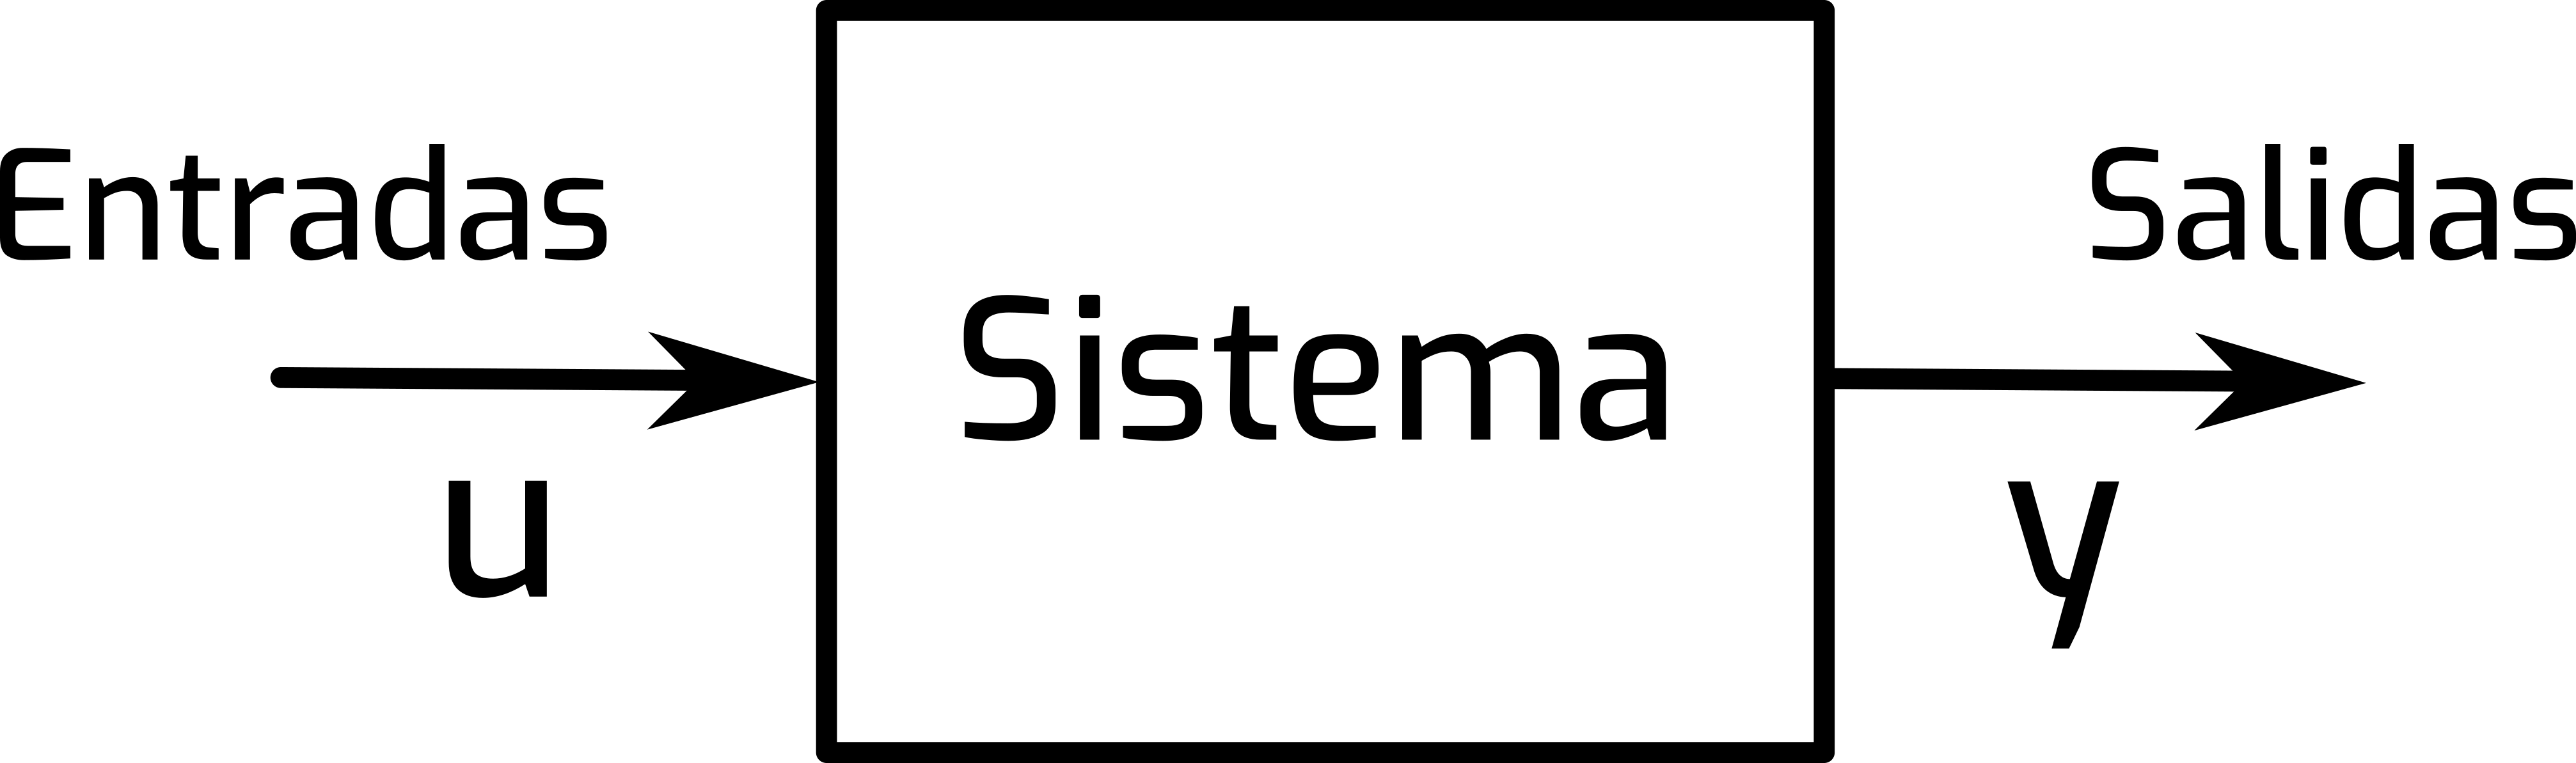
\includegraphics[scale=0.3]{Capitulo3/figs/diagSis.png} 
	\caption{Representación de un sistema como un bloque con sus entradas y salidas}
	\label{dSis}
\end{figure}

En el caso de robots que se desplazan libremente por un espacio de trabajo, tales como los destinados a tareas de pintado, traslado de objetos de un punto a otro, corte por rayo láser, etc, la salida del sistema $\boldsymbol{\mathit{y}}$ puede corresponder simplemente a las posiciones y velocidades articulares, denotadas comunmente con la letra $\boldsymbol{\mathit{q}}$ y  $\boldsymbol{\mathit{\dot{q}}}$, respectivamente, o tambien la posición y orientación del efector final o herramienta.\\

\begin{figure}[h!]
	\centering
	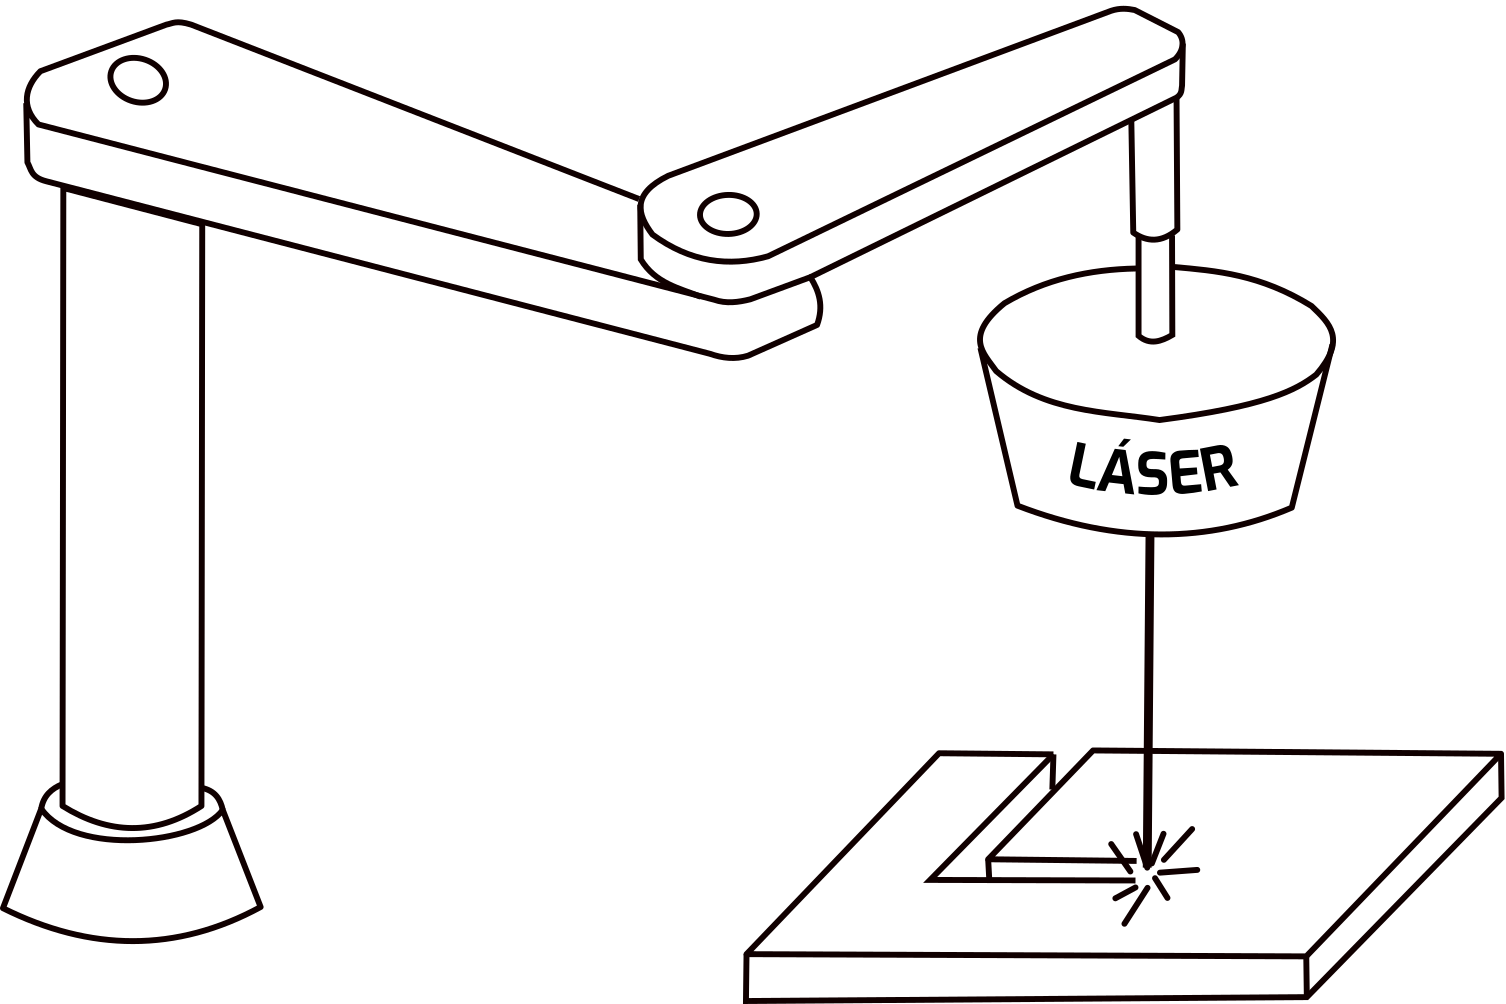
\includegraphics[scale=0.4]{Capitulo3/figs/robotLaser.png} 
	\caption{Robot en movimiento libre}
	\label{laser}
\end{figure}

Para robots manipuladores como el mostrado esquemáticamente en la Figura \ref{gis} que involucra su interacción con el medio ambiente por contacto físico para lograr tareas como pulido de superficies, desbastado de materiales, ensamble de alta precisión, etc., la salida $\boldsymbol{\mathit{y}}$ puede incluir los pares y fuerzas $\boldsymbol{\mathit{f}}$ ejercidos por el efector final del robot sobre su medio ambiente.
\\

\begin{figure}[h!]
	\centering
	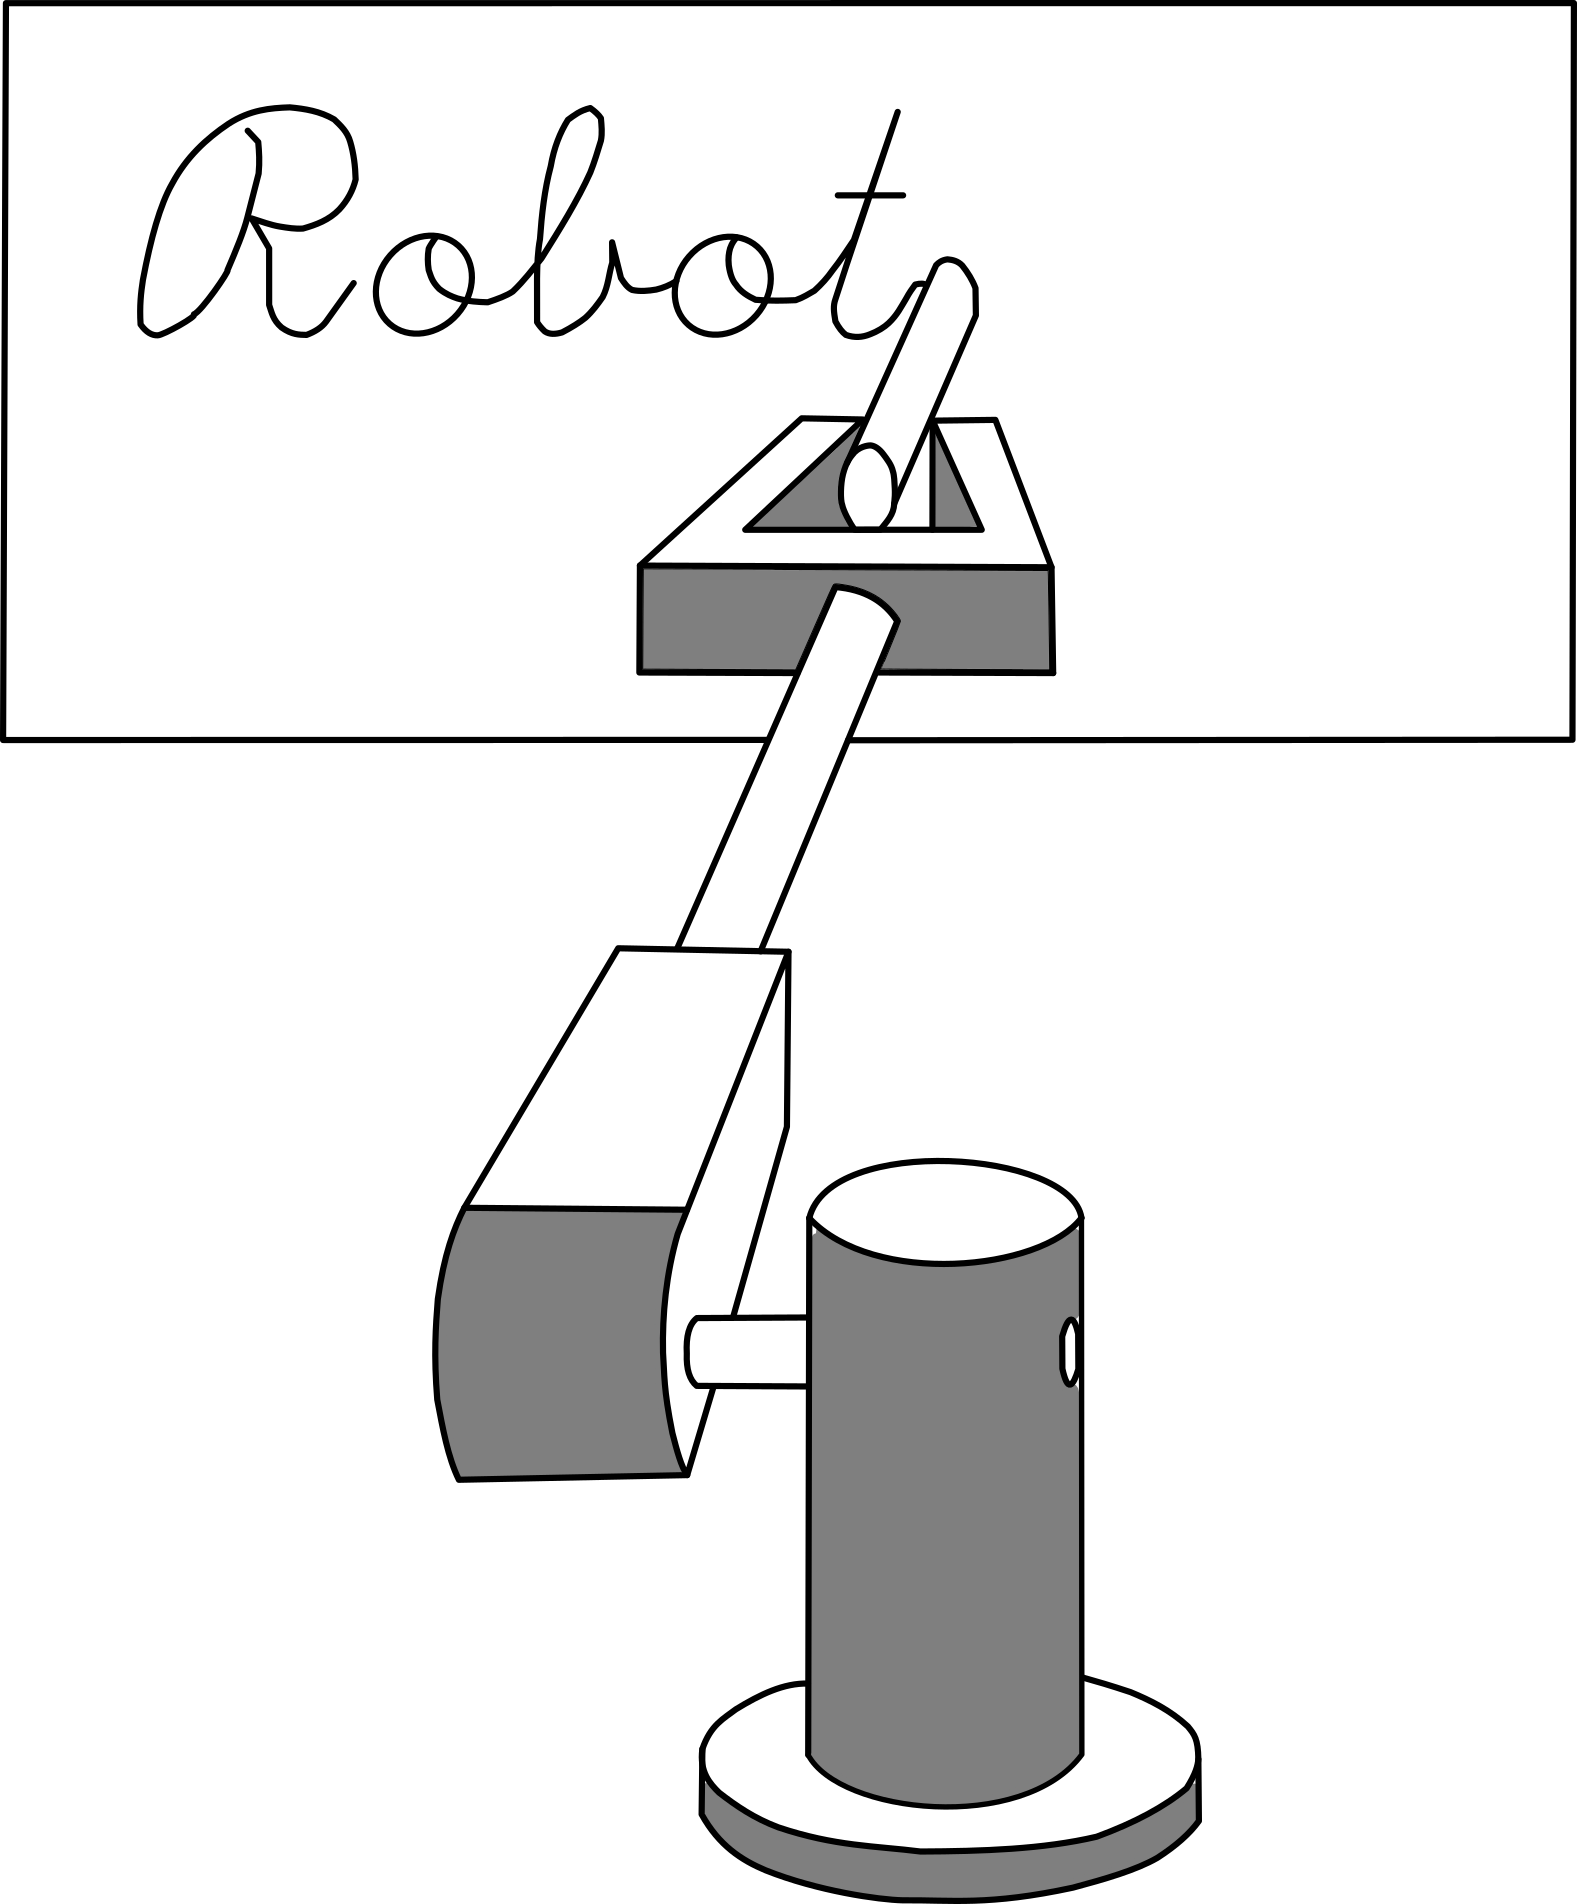
\includegraphics[scale=0.75]{Capitulo3/figs/robotGis.png} 
	\caption{Robot en interacción con el medio ambiente}
	\label{gis}
\end{figure}

De los ejemplos anteriores se desprende que la salida $\boldsymbol{\mathit{y}}$ correspondiente a un robot -asociado a una clase de tareas- en general puede tener la forma funcional:

 $$\boldsymbol{y=y(q,\dot{q},f)}$$
 \linebreak
Por otro lado, las variables de entrada, aquellas que pueden ser modificadas para alterar la evolución de las salidas, son básicamente los pares y fuerzas $\boldsymbol{\tau}$ aplicados por los accionadores sobre las articulaciones del robot. \newpage
La Figura \ref{dBloq} muestra el diagrama de bloques correspondiente al caso donde las posiciones y velocidades articulares $\boldsymbol{\mathit{q}}$ y  $\boldsymbol{\mathit{\dot{q}}}$ son salidas del robot, es decir:

$$\boldsymbol{y=y(q,\dot{q},f)}= \begin{bmatrix}
\boldsymbol{\mathit{q}}\\
\boldsymbol{\mathit{\dot{q}}}
\end{bmatrix}$$
\linebreak
mientras $\boldsymbol{\tau}$ es su entrada. En esta situación podemos notar que para robots con $\mathit{n}$, se tendrán en general $\mathit{2n}$ salidas y $\mathit{n}$ entradas.

\begin{figure}[h!]
	\centering
	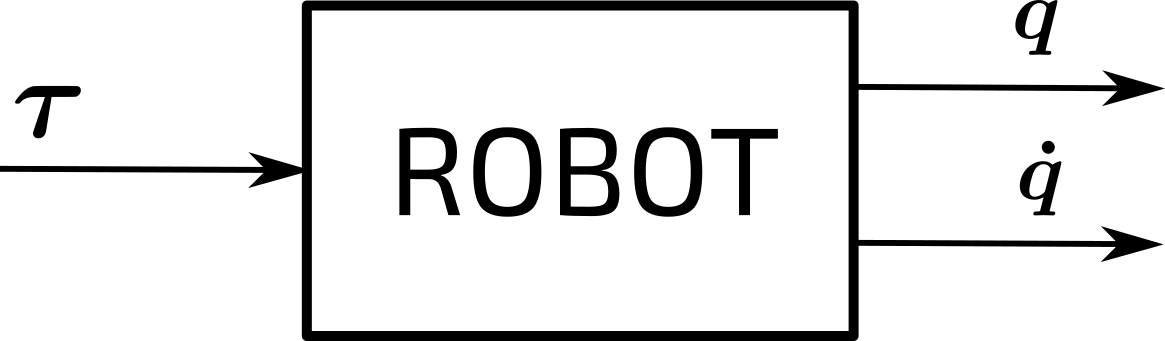
\includegraphics[scale=0.5]{Capitulo3/figs/diagBloq.png} 
	\caption{Diagrama de bloques}
	\label{dBloq}
\end{figure}

\subsection{Modelado dinámico}

En esta etapa se procede a determinar la regla matemática que vincula las variables de entrada y salida del sistema. Generalmente, dicha caracterización matemática se expresa por medio de ecuaciones diferenciales. El modelo matemático del sistema a controlar se obtiene tradicionalmente por una de las dos técnicas siguientes:

\begin{itemize}
	\item \textit{Analítica.} Este procedimiento se basa en las ecuaciones de la física que rigen el comportamiento del sistema. Con esta metodología se puede obtener un modelo matemático preciso a condición de dominar las leyes de la física que están involucradas en el sistema.
	\item \textit{Experimental.} Este procedimiento requiere una serie de datos experimentales del sistema. Frecuentemente se trata de examinar el comportamiento del sistema ante entradas específicas. Su obtención es mas sencilla y se puede obtener en un corto espacio de tiempo, sin embargo, el modelo obtenido es, en general, mas impreciso que el conseguido a partir del metodo analítico. 
\end{itemize}

En algunas ocasiones, en esta etapa se procede a una simplificación del modelo del sistema que se desea controlar con el objetivo de obtener posteriormente un sistema de control relativamente sencillo. Sin embargo esta etapa puede tener al desventaja de dar como resultado un sistema de control que no funcione adecuadamente, fenómeno conocido como \textit{falta de robustez.}\\

En otras ocasiones, después de la etapa de modelado se continúa con la etapa de \textit{identificación paramétrica} con la cual se pretende obtener los valores numéricos de diversos parámetros contenidos en el modelo dinámico. Esto puede llevarse acabo mediante técnicas que emplea mediciones de las entradas y salidas del sistema a controlar.\\

El modelado dinámico de robots manipuladores se realiza tradicionalmente de forma analítica, esto es, a partir de las leyes de la física. Debido a la naturaleza mecánica de los robots manipuladores, las leyes de la física involucradas son simplemente las leyes de la mecánica. Desde el punto de vista de los sistemas dinámicos, un robot manipulador de \textit{n} g.d.l puede ser considerado como un sistema no lineal multivariable, teniendo \textit{n} entradas (los pares y fuerzas $\boldsymbol{\tau}$ que son aplicados en las articulaciones por medio de actuadores electromecánicos, hidráulicos o neumaticos) y \textit{2n} variables de estado, normalmente asociadas a las \textit{n} posiciones $\boldsymbol{\mathit{q}}$ y \textit{n} velocidades $\boldsymbol{\mathit{\dot{q}}}$ articulares. La Figura \ref{dBloq} muestra el diagrama de bloques correspondiente suponiendo que las variables de estado corresponden también a las salidas. \\

Los modelos dinámicos de los robots manipuladores son en general caracterizados por ecuaciones diferenciales ordinarias no lineales y autónomas. Este hecho tiene como consecuencia que las técnicas de diseño tradicionales para el control de sistemas lineales tengan una aplicación limitada en la obtención de controladores de alto desempeño para robots manipuladores. Si sumamos lo anterior dicho con los requerimientos actuales de alta precisión y rapidez en los movimientos de los robots, se hace necesario el uso de técnicas mas elaboradas de control con mayores prestaciones. Esta clase de sistemas de control pueden incluir, por ejemplo, controles no lineales y controles adaptables.\\
\subsection{Especificaciones de control}

%Ejemplo de cita \citep{texbook}


%%%%%%%%%%%%%%%%%%%%%%%%%%%%%%%%%%%%%%%%%%%%%%%%%%%%%%%%%%%%%%%%%%%%%%%%%
%                          Modelado                                     %
%%%%%%%%%%%%%%%%%%%%%%%%%%%%%%%%%%%%%%%%%%%%%%%%%%%%%%%%%%%%%%%%%%%%%%%%%
\section{Esquemas de control}

\subsection{PID}

\section{Control por par calculado}

\section{Diseño del Controlador}
Antes de comenzar, se definen  en la tabla ~\ref{tab:tabla} los parámetros y variables utilizadas

%%%%%%%%Tabla Nombres de parámetros
\begin{table}[htdp]                             %Inicia el entorno table debajo del texto
\centering\                                     %   centra la tabla
\begin{tabular}{||c | c ||}                     %inicia entorno tabular con doble línea en las orillas, 2 columnas con el contenido centrado (c)
\hline                                          %inserta línea horizontal
\hline
Nombre Parámetro/Variable & Símbolo\\
\hline
\hline
Masa del péndulo & $m$ \\
\hline
Masa del carro & $M$\\
\hline
Distancia del eje de giro al centro de masa & $l$ \\
\hline
Aceleración gravitatoria & $g$ \\
\hline
Momento de inercia péndulo respecto del eje de giro& $J$ \\
\hline
Ángulo del péndulo respecto del eje vertical & $\theta$\\
\hline
Velocidad angular del péndulo & $\dot{\theta}$, $\omega$\\
\hline
Distancia del carro respecto al centro del riel & x\\
\hline
Velocidad del carro & $\dot{x}$, $v$\\
\hline
\hline
\end{tabular}
\caption[Tabla 1]{\textbf{Parámetros dinámicos del carro-péndulo} - Estos son los valores de parámetros utilizados en el diseño y las simulaciones, corresponden a los valores reales.}
\label{tab:tabla}                              %etiqueta para referencia
\end{table}
